\begin{frame}{}
    \LARGE VAE: \textbf{Introduction}
\end{frame}


\begin{frame}[allowframebreaks]{Introduction}
  \begin{itemize}
    \item We want a \textbf{generative model}, which given a prior $\mathbf{z}$ outputs a new sample from data.
    \item To make the latent space $Z$ continuous, let's choose it to be Gaussian
    \item So now, we want to estimate the true parameters $\theta^*$ of this generative model.
    \begin{figure}
        \centering
        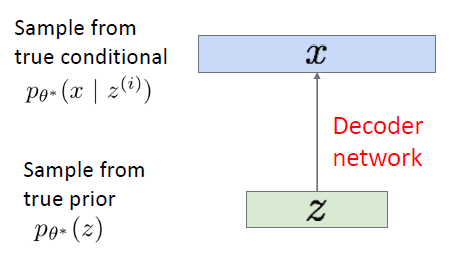
\includegraphics[height=0.5\textheight, width=\textwidth, keepaspectratio]{./images/vae/abstract_model.png}
    \end{figure}
\end{itemize}

\framebreak

\begin{itemize}
  \item \textbf{Probabilistic Encoder:} Instead of encoding an input \( x \) to a fixed point \( z \), the encoder learns a distribution over the latent variable \( z \) conditioned on the input:
  \[ q(z \mid x) \]
  Typically, this is a multivariate Gaussian with parameters \( \mu(x) \) and \( \sigma(x) \) learned by a neural network.

  \framebreak
  
  \item \textbf{Probabilistic Decoder:} Given a sample \( z \) from the latent distribution, the decoder reconstructs the input by modeling:
  \[
  p(x \mid z)
  \]
  This allows for generating new data by sampling from the latent space.

  \framebreak

  \item \textbf{Latent Space:}
    \begin{itemize}
      \item The model learns a smooth, continuous space for \( z \).
      \item Similar data points end up close together in this space.
      \item This helps the model understand the main patterns in the data.
    \end{itemize}
\end{itemize}

\framebreak

\textbf{Objectives and Training}: The training objective of a VAE is to maximize the \textbf{Evidence Lower Bound (ELBO)}:
% \begin{itemize}
%   \item \textbf{Training Objective:} The model is trained to maximize the Evidence Lower Bound (ELBO), which balances reconstruction accuracy and the complexity of the latent space.
%   \[
%   \mathcal{L} = \mathbb{E}_{q(z \mid x)}[\log p(x \mid z)] - D_{KL}(q(z \mid x) \| p(z))
%   \]
%   where \( D_{KL} \) is the Kullback-Leibler divergence between the learned distribution and a prior distribution \( p(z) \).

%   \item \textbf{Reparameterization Trick:} To allow backpropagation through the stochastic sampling process, we use a reparameterization trick that expresses \( z \) as a deterministic function of \( x \) and a random variable \( \epsilon \):
%   \[
%   z = \mu(x) + \sigma(x) \odot \epsilon
%   \]
%   where \( \epsilon \sim N(0, I) \).
%   \item \textbf{Generative Model:} After training, the VAE can generate new samples by sampling from the prior \( p(z) \) and passing the samples through the decoder.
% \end{itemize}


\[
\log p(x) \geq \mathbb{E}_{q(z|x)}[\log p(x|z)] - D_{\mathrm{KL}}(q(z|x) \| p(z))
\]

\begin{itemize}
  \item The first term, \( \mathbb{E}_{q(z|x)}[\log p(x|z)] \), encourages accurate reconstruction.
  \item The second term, \( D_{\mathrm{KL}}(q(z|x) \| p(z)) \), regularizes the latent space by making the approximate posterior \( q(z|x) \) close to the prior \( p(z) \), usually \( \mathcal{N}(0, I) \).
\end{itemize}

\framebreak

\textbf{Why Use VAEs?}: 
\begin{itemize}
  \item Enable generative modeling: generate new samples by sampling from the latent distribution.
  \item Learn smooth, structured, and interpretable latent representations.
  \item Provide a principled probabilistic framework for inference and generation.
\end{itemize}

\end{frame}